\documentclass{article}

\usepackage{amsmath}
\usepackage{amssymb}
\usepackage{geometry}
\usepackage{array}
\usepackage{graphicx}
\usepackage{booktabs}
\usepackage{multicol} 
\usepackage{amsfonts} 
\usepackage{pgfplots}

% the exam will have one question from modulation 
% and one from sampling

\geometry{margin=0.2in}
\setlength{\columnsep}{0.2in} 

\begin{document}
\begin{multicols}{2}

    \noindent\textbf{Sum of Squares}\\
    \begin{equation*}
        \sum_{k=0}^{n} k^2 = \frac{n(n+1)(2n+1)}{6}
    \end{equation*}

    \noindent\textbf{Sum of Geometric Series}\\
    \begin{equation*}
        \sum_{k=0}^{n} ar^k = a\frac{1-r^n}{1-r}
    \end{equation*}

    \noindent\textbf{Sum of Weighted Geometric Series}\\
    \begin{equation*}
        \sum_{k=0}^{n} kr^k = r\frac{1- (n + 1)r^n +nr^{n + 1}}{(1-r)^2}
    \end{equation*}

    \noindent\textbf{Memoryless}\\
    A \emph{memoryless} system's output depends only on the input at time
    \( t \) (or \( n \) for discrete-time systems), and not on past or
    future states. For example, \( y(t) = 2x(t) \) is memoryless, while
    \( y[n] = x[n-1] \) has memory.

    \noindent\textbf{Linearity}\\
    A system is \emph{linear} if it satisfies superposition and homogeneity.
    Formally, for any inputs \( x_1(t) \rightarrow y_1(t) \) and
    \( x_2(t) \rightarrow y_2(t) \), and constants \( a, b \), the system
    satisfies:
    \[
        S\{a x_1(t) + b x_2(t)\} = a S\{x_1(t)\} + b S\{x_2(t)\} = a y_1(t) + b y_2(t).
    \]
    An example is \( y(t) = kx(t) \), where \( k \) is a constant.

    \noindent\textbf{Time Invariance}\\
    A system is \emph{time invariant} if a time shift in the input results in
    an identical shift in the output. For a discrete-time system \( S \), if:
    \[
        x[n] \rightarrow y[n],
    \]
    then for any integer \( n_0 \):
    \[
        x[n - n_0] \rightarrow y[n - n_0].
    \]

    \noindent\textbf{Linear Time Invariance}\\
    An LTI system satisfies both linearity and time invariance.
    LTI systems are fully characterized by their impulse response
    \( h(t) \) or \( h[n] \), enabling analysis via convolution:
    \( y(t) = x(t) * h(t) \). The impulse response is found by
    plugging in $\delta(t)$ or $\delta[n]$ to the system. The result
    is the impulse response. Mathematically,
    \begin{align*}
        h(t) & = S(\delta(t))  \\
        h[n] & = S(\delta[n]).
    \end{align*}

    \noindent\textbf{Causality}\\
    A system is \emph{causal} if its output at time \( t \) depends
    only on present and past inputs.
    For causal systems, the impulse response must be 0 for values of $n$ ($t$)
    less than 0.

    \noindent\textbf{Stability}\\
    A system is \emph{stable} if bounded inputs produce
    bounded outputs. Formally, there exist constants \( B, M > 0 \)
    such that:
    \[
        |x(t)| < B \ \forall t \implies |y(t)| < M \ \forall t.
    \]
    \[
        \sum_{k=-\infty}^{\infty} |h[k]| < \infty.
    \]
    \[
        \int_{-\infty}^{\infty} |h(\tau)| d\tau < \infty.
    \]

    \noindent\textbf{HRCE}
    \[
        x_k(t) = e^{jk\omega_0 t}, k \in \mathbb{Z}.
    \]
    \[
        x_k[n] = e^{jk\omega_0 n}, k \in \{0, 1, ..., N\}.
    \]

    \noindent\textbf{Energy}
    \begin{align*}
        E & = \int_{t_1}^{t_2} |x(t)|^2 dt                     \\
          & = \int_{t_1}^{t_2} (x_{Re}(t)^2 + x_{Im}(t)^2) dt.
    \end{align*}
    \begin{align*}
        E & = \sum_{n=n_1}^{n_2} |x[n]|^2                     \\
          & = \sum_{n=n_1}^{n_2} (x_{Re}[n]^2 + x_{Im}[n]^2).
    \end{align*}

    \noindent\textbf{Power}
    \[
        P_{avg} = \frac{1}{t_2 - t_1} \int_{t_1}^{t_2} |x(t)|^2 dt.
    \]
    \[
        P_{avg} = \frac{1}{n_2 - n_1 + 1} \sum_{n=n_1}^{n_2} |x[n]|^2.
    \]
    \[
        P_{\infty} = \lim_{T \rightarrow \infty} \frac{1}{2T} \int_{-T}^{T} |x(t)|^2 dt
    \]
    \[
        P_{\infty} = \lim_{N \rightarrow \infty} \frac{1}{2N + 1} \sum_{n=-N}^{N} |x[n]|^2
    \]

    \noindent\textbf{Poisson Summation Formula}
    \begin{align*}
        X(j\omega)     & = 2\pi\sum_{k=-\infty}^{\infty} a_k \delta\left( \omega - \frac{2\pi k}{T} \right) \\
        X(e^{j\omega}) & = 2\pi\sum_{k=-\infty}^{\infty} a_k \delta\left( \omega - \frac{2\pi k}{N} \right)
    \end{align*}

    \noindent\textbf{Analysis Equation}
    \begin{align*}
        X(j\omega)     & = \int_{-\infty}^{\infty} x(t) e^{-j\omega t} dt \\
        X(e^{j\omega}) & = \sum_{n=-\infty}^{\infty} x[n] e^{-j\omega n}
    \end{align*}

    \noindent\textbf{Synthesis Equation}
    \begin{align*}
        a_k  & = \frac{1}{T} \int_{<T>} x(t) e^{-jk\frac{2\pi}{T} t} dt                  \\
        x(t) & = \sum_{k=-\infty}^{\infty} a_k e^{jk\frac{2\pi}{T} t}                    \\
             & = \frac{1}{2\pi} \int_{-\infty}^{\infty} X(j\omega) e^{j\omega t} d\omega \\
        a_k  & = \frac{1}{N} \sum_{n=<N>} x[n] e^{-jk\frac{2\pi}{N}n}                    \\
        x[n] & = \sum_{k=<N>} a_k e^{jk\frac{2\pi}{N} n}                                 \\
             & = \frac{1}{2\pi} \int_{-\pi}^{\pi} X(e^{j\omega}) e^{j\omega n} d\omega
    \end{align*}

    \noindent\textbf{Symmetry Properties} \\
    If $x(t)$ is real, then $|X(j\omega)|$ is even and
    $\angle X(j\omega)$ is odd. Moreover, if $x(t)$ is real
    and even, then $X(j\omega)$ must be purely real and even,
    and if $x(t)$ is real and odd, $X(j\omega)$ is purely
    imaginary and odd.

    \noindent\textbf{Duality Property}
    \[ \label{eq:duality}
        \mathcal{F}\left\{ X(t) \right\} = 2\pi x(-\omega).
    \]

    \noindent\textbf{Modulation Property} \\
    \begin{align*}
        x(t)\cos(\omega_0 t) & \overset{\mathcal{F}}{\leftrightarrow} \frac{1}{2}\left( X(j(\omega-\omega_0)) + X(j(\omega+\omega_0))\right)          \\
        x[n]\cos(\omega_0 n) & \overset{\mathcal{F}}{\leftrightarrow}  \frac{1}{2}\left( X(e^{j(\omega-\omega_0)}) + X(e^{j(\omega+\omega_0)})\right)
    \end{align*}

    \noindent\textbf{Amplitude Modulation}\\
    Modulate $x(t)$ with carrier $e^{j\omega_c t}$ or $\cos(\omega_c t)$.
    For complex exponential modulation,
    \[
        x_{\text{AM}}(t) = x(t) e^{j\omega_c t}
    \]
    In frequency domain:
    \[
        X_{\text{AM}}(j\omega) = X(j(\omega - \omega_c))
    \]
    To demodulate, multiply by $e^{-j\omega_c t}$ and lowpass filter.
    For sinusoidal modulation, modulate $x(t)$ with $\cos(\omega_c t)$:
    \[
        x_{\text{AM}}(t) = x(t) \cos(\omega_c t)
    \]
    In frequency domain:
    \[
        X_{\text{AM}}(j\omega) = \frac{1}{2}\left[X(j(\omega-\omega_c)) + X(j(\omega+\omega_c))\right]
    \]
    To demodulate, multiply received AM signal by $\cos(\omega_c t)$ and lowpass filter:
    \[
        y(t) = x_{\text{AM}}(t) \cdot \cos(\omega_c t)
    \]
    This yields terms at baseband and $2\omega_c$; lowpass filtering recovers $x(t)$.
    Alternatively, for $x(t)$ slowly varying and $x_{\text{AM}}(t) = [A + x(t)]\cos(\omega_c t)$,
    the envelope (magnitude) of $x_{\text{AM}}(t)$ approximates $A + x(t)$.

    \noindent\textbf{Frequency Division Multiplexing}\\
    Multiple signals $x_k(t)$ modulated onto different carrier frequencies $\omega_k$:
    \[
        s(t) = \sum_{k} x_k(t) \cos(\omega_k t)
    \]
    Each $x_k(t)$ occupies a unique frequency band; signals are separated at the receiver by bandpass filtering and demodulation.

    \noindent\textbf{Frequency Spectrum}\\
    The plot of the magnitude of a signal's Fourier transform is its
    frequency spectrum.
    For example, the Fourier transform of $\cos(2 t)$ is
    $\pi \left[\delta(\omega - 2) + \delta(\omega + 2)\right]$
    so its frequency spectrum is
    \begin{center}
        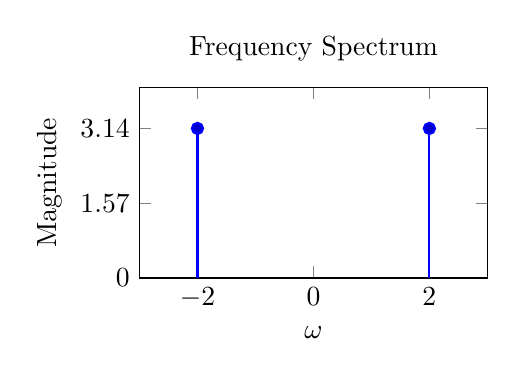
\begin{tikzpicture}
            \begin{axis}[
                    width=6cm, height=4cm,
                    xlabel={$\omega$},
                    ylabel={Magnitude},
                    title={Frequency Spectrum},
                    ymin=0, ymax=4,
                    xmin=-3, xmax=3,
                    xtick={-2, 0, 2},
                    ytick={0,pi/2,pi},
                ]
                % Two impulses at f=5 and f=15 (for illustration)
                \addplot+[ycomb, mark=*, thick, blue] coordinates {(-2,pi) (2,pi)};
            \end{axis}
        \end{tikzpicture}
    \end{center}

    \noindent\textbf{LTI System Invertibility Criterion} \\
    An LTI system with frequency response $H(j\omega)$ (CT) or $H(e^{j\omega})$ (DT) is
    invertible if and only if $H(j\omega) \neq 0$ for all $\omega$ (CT) or $H(e^{j\omega})
        \neq 0$ for all $\omega \in [-\pi, \pi]$ (DT). If the system is invertible, then the
    inverse is $\frac{1}{H(j\omega)}$ (CT) or $\frac{1}{H(e^{j\omega})}$ (DT).

    \noindent\textbf{LTI System Input/Output}
    \begin{align*}
        Y(j\omega)     & = H(j\omega)X(j\omega)         \\
        Y(e^{j\omega}) & = H(e^{j\omega})X(e^{j\omega})
    \end{align*}

    \noindent\textbf{LTI with Periodic Complex Exponential Input} \\
    Let the input to an LTI system be $e^{j\omega_0 t}$, and let the
    impulse response be $h(t)$. Then
    \[
        y(t) = H(j\omega_0)e^{j\omega_0 t}.
    \]

    \noindent\textbf{Differential Equations} \\
    For a system described by:
    \[
        \sum_{k=0}^{N} a_k \frac{d^k y(t)}{dt^k} = \sum_{k=0}^{M} b_k \frac{d^k x(t)}{dt^k}
    \]
    The frequency response is:
    \[ \label{eq:diff_eq_Hjw}
        H(j\omega) = \frac{Y(j\omega)}{X(j\omega)} = \frac{\sum_{k=0}^{M} b_k (j\omega)^k}{\sum_{k=0}^{N} a_k (j\omega)^k}
    \]

    \noindent\textbf{Difference Equations} \\
    For a system described by:
    \[
        \sum_{k=0}^{N} a_k y[n-k] = \sum_{k=0}^{M} b_k x[n-k]
    \]
    The frequency response is:
    \[ \label{eq:diff_eq_Hejomega}
        H(e^{j\omega}) = \frac{Y(e^{j\omega})}{X(e^{j\omega})} = \frac{\sum_{k=0}^{M} b_k e^{-j\omega k}}{\sum_{k=0}^{N} a_k e^{-j\omega k}}
    \]

    \noindent\textbf{Sampling Theorem} \\
    Let $x(t)$ be a band-limited signal with
    $X(j\omega) = 0$ for $|\omega| > \omega_M$.
    Then $x(t)$ is uniquely determined by its samples
    $x(nT)$, $n = 0, \pm 1, \pm 2, \dots$ if
    \begin{equation*}
        \omega_s > 2 \omega_M,
    \end{equation*}
    where
    \begin{equation*}
        \omega_s = \frac{2\pi}{T}.
    \end{equation*}
    Given these samples, we can reconstruct
    $x(t)$ by generating a periodic impulse
    train in which succesive impulses have amplitudes that are
    successive sample values. This impulse train is
    then processed through an ideal lowpass filter
    with gain $T$ and cutoff frequency greater than $\omega_M$ and
    less than $\omega_s - \omega_M$.
    The resulting output signal will exactly equal $x(t)$.
    If $\omega_s<2\omega_M$, spectral replicas overlap (aliasing),
    and $x(t)$ cannot be recovered exactly, though samples coincide:
    $x_r(nT)=x(nT)$.

    \noindent\textbf{Interpolation and Holds}\\
    Reconstruction via LTI filters or "holds":
    \begin{itemize}
        \item Zero-Order Hold (ZOH): impulse response $h_0(t)=u(t)-u(t-T)$, output holds each sample constant.
        \item First-Order Hold (Linear Interpolation): triangular impulse $h_1(t)=\frac{1}{T}(1-\frac{|t|}{T})$ for $|t|<T$, cascaded ZOHs.
        \item Ideal Band-Limited Interpolation (Sinc): $h_{\rm ideal}(t)=\frac{\omega_s}{\pi}~\mathrm{sinc}(\omega_s t/2)$ gives perfect reconstruction when conditions met.
    \end{itemize}

    \begin{table*}[ht]
        \centering
        \caption{Properties of Fourier Transforms}
        \label{tab:fourier_transform_properties}
        \small
        \begin{tabular}{@{}lllll@{}}
            \toprule
            \textbf{Property}  & \textbf{CT Time Domain}             & \textbf{CT Frequency Domain}                                  & \textbf{DT Time Domain}            & \textbf{DT Frequency Domain}                                                                            \\
            \midrule
            Linearity          & $A x_1(t) + B x_2(t)$               & $A X_1(j\omega) + B X_2(j\omega)$                             & $A x_1[n] + B x_2[n]$              & $A X_1(e^{j\omega}) + B X_2(e^{j\omega})$                                                               \\ [1mm]
            Time Shifting      & $x(t - t_0)$                        & $X(j\omega)e^{-j\omega t_0}$                                  & $x[n - n_0]$                       & $X(e^{j\omega})e^{-j\omega n_0}$                                                                        \\ [1mm]
            Frequency Shifting & $x(t)e^{j\omega_0 t}$               & $X(j(\omega - \omega_0))$                                     & $x[n]e^{j\omega_0 n}$              & $X(e^{j(\omega - \omega_0)})$                                                                           \\ [1mm]
            Time Scaling       & $x(at)$, $a \neq 0$                 & $\frac{1}{|a|}X\left(\frac{j\omega}{a}\right)$                & ---                                & ---                                                                                                     \\ [1mm]
            Time Reversal      & $x(-t)$                             & $X(-j\omega)$                                                 & $x[-n]$                            & $X(e^{-j\omega})$                                                                                       \\ [1mm]
            Conjugation        & $x^*(t)$                            & $X^*(-j\omega)$                                               & $x^*[n]$                           & $X^*(e^{-j\omega})$                                                                                     \\ [1mm]
            Differentiation    & $\frac{d^n}{dt^n}x(t)$              & $(j\omega)^n X(j\omega)$                                      & $x[n] - x[n-1]$                    & $(1 - e^{-j\omega})X(e^{j\omega})$                                                                      \\ [1mm]
            Integration        & $\int_{-\infty}^t x(\tau) d\tau$    & $\frac{X(j\omega)}{j\omega} + \pi X(0)\delta(\omega)$         & $\sum_{k=-\infty}^n x[k]$          & $\frac{X(e^{j\omega})}{1-e^{-j\omega}} + \pi X(e^{j0})\sum_{k=-\infty}^{\infty}\delta(\omega - 2\pi k)$ \\ [1mm]
            Convolution        & $(x_1 * x_2)(t)$                    & $X_1(j\omega) X_2(j\omega)$                                   & $(x_1 * x_2)[n]$                   & $X_1(e^{j\omega}) X_2(e^{j\omega})$                                                                     \\ [1mm]
            Multiplication     & $x_1(t)x_2(t)$                      & $\frac{1}{2\pi}(X_1 * X_2)(j\omega)$                          & $x_1[n]x_2[n]$                     & $\frac{1}{2\pi}\int_{-\pi}^{\pi} X_1(e^{j\theta}) X_2(e^{j(\omega-\theta)}) d\theta$                    \\ [1mm]
            Parseval's Theorem & $\int_{-\infty}^\infty |x(t)|^2 dt$ & $\frac{1}{2\pi} \int_{-\infty}^\infty |X(j\omega)|^2 d\omega$ & $\sum_{n=-\infty}^\infty |x[n]|^2$ & $\frac{1}{2\pi} \int_{-\pi}^{\pi} |X(e^{j\omega})|^2 d\omega$                                           \\
            \bottomrule
        \end{tabular}
    \end{table*}

    % add line for Fourier transform of e^{j\omega_0 t}
    \begin{table*}[ht]
        \centering
        \caption{Fourier Transform Pairs}
        \label{tab:fourier_transform_pairs}
        \small
        \begin{tabular}{@{}llll@{}}
            \toprule
            \textbf{CT Time Domain} $x(t)$                                 & \textbf{CT Fourier Transform} $X(j\omega)$                                    & \textbf{DT Time Domain} $x[n]$                                          & \textbf{DT Fourier Transform} $X(e^{j\omega})$                                                                                      \\
            \midrule
            $\delta(t)$                                                    & $1$                                                                           & $\delta[n]$                                                             & $1$                                                                                                                                 \\ [1mm]
            $1$                                                            & $2\pi\,\delta(\omega)$                                                        & $1$                                                                     & $2\pi\,\sum_{k=-\infty}^{\infty}\delta(\omega-2\pi k)$                                                                              \\ [1mm]
            $u(t)$                                                         & $\pi\,\delta(\omega) + \frac{1}{j\omega}$                                     & $u[n]$                                                                  & $\frac{1}{1-e^{-j\omega}} + \pi \sum_{k=-\infty}^{\infty} \delta(\omega - 2\pi k)$                                                  \\ [1mm]
            $e^{-at}u(t),\quad \Re(a)>0$                                   & $\dfrac{1}{a+j\omega}$                                                        & $a^n u[n],\quad |a|<1$                                                  & $\dfrac{1}{1-ae^{-j\omega}}$                                                                                                        \\ [1mm]
            $e^{-a|t|},\, a>0$                                             & $\dfrac{2a}{a^2+\omega^2}$                                                    & $a^{|n|},\quad |a|<1$                                                   & $\dfrac{1-a^2}{1-2a\cos\omega+a^2}$                                                                                                 \\ [1mm]
            $t e^{-at} u(t),\quad \Re(a)<0$                                & $\dfrac{1}{(a+j\omega)^2}$                                                    & ---                                                                     & ---                                                                                                                                 \\ [1mm]
            $\frac{t^{n-1}}{(n-1)!}e^{-a t}u(t),\;\Re(a)<0$                & $\frac{1}{(a + j\omega)^n}$                                                   & $n\,a^n\,u[n],\;|a|<1$                                                  & $\frac{a\,e^{-j\omega}}{\bigl(1 - a\,e^{-j\omega}\bigr)^2}$                                                                         \\ [1mm]
            $\cos(\omega_0 t)$                                             & $\pi\Bigl[\delta(\omega-\omega_0) + \delta(\omega+\omega_0)\Bigr]$            & $\cos(\omega_0 n)$                                                      & $\pi\,\sum_{k=-\infty}^{\infty}\Bigl[\delta(\omega-\omega_0-2\pi k) + \delta(\omega+\omega_0-2\pi k)\Bigr]$                         \\ [1mm]
            $\sin(\omega_0 t)$                                             & $\dfrac{\pi}{j}\Bigl[\delta(\omega-\omega_0) - \delta(\omega+\omega_0)\Bigr]$ & $\sin(\omega_0 n)$                                                      & $\dfrac{\pi}{j}\,\sum_{k=-\infty}^{\infty}\Bigl[\delta(\omega-\omega_0-2\pi k) - \delta(\omega+\omega_0-2\pi k)\Bigr]$              \\ [1mm]
            $\begin{cases} 1, & |t| \le T/2 \\ 0, & |t| > T/2 \end{cases}$ & $2\frac{\sin\left(\frac{\omega T}{2}\right)}{\omega}$                         & $\begin{cases} 1, & 0 \le n \le N \\ 0, & \text{otherwise} \end{cases}$ & $\dfrac{\sin\Bigl(\omega (N+1)/2\Bigr)}{\sin\Bigl(\omega/2\Bigr)}\,e^{-j\omega N/2}$                                                \\ [1mm]
            $\frac{\sin\left(Wt\right)}{\pi t}$                            & $\begin{cases} 1, & |\omega| \le W \\ 0, & |\omega| > W \end{cases}$          & $\frac{\sin\left(Wn\right)}{\pi n}$                                     & $\begin{cases} 1, & 0 \leq |\omega| \le W \\ 0, & W < |\omega| \leq \pi \end{cases}$, $X(e^{j\omega})$ periodic with period $2\pi$. \\ [1mm]
            \bottomrule
        \end{tabular}
    \end{table*}

    \begin{table*}[ht]
        \centering
        \caption{Properties of Fourier Series}
        \label{tab:fourier_series_properties}
        \small
        \begin{tabular}{@{}lllll@{}}
            \toprule
            \textbf{Property}    & \textbf{CT Time Domain}                               & \textbf{CT Frequency Domain} ($a_k$)                            & \textbf{DT Time Domain}                       & \textbf{DT Frequency Domain} ($a_k$)                                       \\
            \midrule
            Linearity            & $A x_1(t) + B x_2(t)$                                 & $A a_k + B b_k$                                                 & $A\,x_1[n] + B\,x_2[n]$                       & $A\,a_k + B\,b_k$                                                          \\ [1mm]
            Time Shifting        & $x(t - t_0)$                                          & $a_k e^{-j k \omega_0 t_0}$                                     & $x[n-n_0]$                                    & $a_k\,e^{-j\frac{2\pi}{N} k n_0}$                                          \\ [1mm]
            Frequency Shifting   & $x(t) e^{j M \omega_0 t}$                             & $a_{k - M}$                                                     & $x[n]\,e^{j\frac{2\pi}{N} M n}$               & $a_{(k-M)\,\mathrm{mod}\,N}$                                               \\ [1mm]
            Time Reversal        & $x(-t)$                                               & $a_{-k}$                                                        & $x[-n]$                                       & $a_{-k}$ (indices mod $N$)                                                 \\ [1mm]
            Conjugation          & $x^*(t)$                                              & $a_{-k}^*$                                                      & $x^*[n]$                                      & $a^*_{-k}$ (indices mod $N$)                                               \\ [1mm]
            Periodic Convolution & $(x \ast y)(t)$                                       & $T a_k b_k$                                                     & $(x\circledast y)[n]$                         & $N a_k\,b_k$                                                               \\ [1mm]
            Multiplication       & $x(t) y(t)$                                           & $\sum_{l=-\infty}^{\infty} a_l b_{k - l}$                       & $x[n]\,y[n]$                                  & $\sum_{m=0}^{N-1} a_m\,b_{(k-m)\,\mathrm{mod}\,N}$                         \\ [1mm]
            Differentiation      & $\frac{d}{dt} x(t)$                                   & $j k \omega_0 a_k$                                              & $x[n]-x[n-1]$                                 & $a_k\Bigl(1-e^{-j\frac{2\pi}{N} k}\Bigr)$                                  \\ [1mm]
            Integration          & $\int x(t) dt$                                        & $\frac{a_k}{j k \omega_0}$ ($a_0 = 0$)                          & ---                                           & ---                                                                        \\ [1mm]
            Parseval's Theorem   & $\frac{1}{T} \int_T |x(t)|^2 dt$                      & $\sum_{k=-\infty}^{\infty} |a_k|^2$                             & $\frac{1}{N}\sum_{n=0}^{N-1}|x[n]|^2$         & $\sum_{k=0}^{N-1}|a_k|^2$                                                  \\ [1mm]
            Running Sum          & $\displaystyle y(t)=\int_{-\infty}^{t}x(\tau)\,d\tau$ & $\displaystyle \frac{a_k}{j\,k\,\omega_0}\quad(k\neq0,\;a_0=0)$ & $\displaystyle y[n]=\sum_{m=-\infty}^{n}x[m]$ & $\displaystyle \frac{a_k}{1 - e^{-j\frac{2\pi}{N}k}}\quad(k\neq0,\;a_0=0)$ \\ [1mm]
            Symmetry (Real)      & $x(t)$ real                                           & $a_k = a_{-k}^*$                                                & $x[n]$ real                                   & $a_k = a_{-k}^*$                                                           \\ [1mm]
            Symmetry (Real+Even) & $x(t)$ real and even                                  & $a_k$ real and even                                             & $x[n]$ real and even                          & $a_k$ real and even                                                        \\ [1mm]
            Symmetry (Real+Odd)  & $x(t)$ real and odd                                   & $a_k$ purely imaginary and odd                                  & $x[n]$ real and odd                           & $a_k$ purely imaginary and odd                                             \\
            \bottomrule
        \end{tabular}
    \end{table*}

\end{multicols}
\end{document}